%Chapter of Background
%Take everything from poster and then add a whole lot
%Explain AE,signing,cipers, types of attack that my app may have to defend against, keys, nonces, 

\chapter{Background}
\label{back}

\section{Cryptography}

Cryptography is the practise of and study of techniques for secure communication in the presence of attackers. To do so, one can use encryption where by messages are encoded in such a way that only authorised parties, or at least parties in possession of the keys, can view them. Hashing, usually packaged within functions, is used to provide message integrity. Digital signatures can be used to provide authentication. There are two main ways of encryption Symmetric Key encryption and Asymmetric Key encryption. In Symmetric Key encryption both parties have the same key which can encrypt and decrypt messages that are sent between them. The problem is that if Bob wants to send an encrypted message to Alice, he must get the private key to her. The key distrubution problem is a well known problem in cryptography and is explained further in section \ref{keydist}. Currently the most secure way for the transmission of private keys is to hand them over in person, in private. This project uses asymmetric key securely encryption and digital signatures.


\subsection{Asymmetric Key Encryption}

To get round the key distribution problem, one can use Asymmetric Key encryption, a visual depiction can be seen in figure \ref{fig:asy}. Asymmetric key encryption involves a private key and a public key, the private key is generally random data and is used to generate a corresponding public key. The public key is mathematically linked to the private key but it is computationally infeasible to calculate the private key back from the public key. This public key can be given out freely and is not a secret. So if Bob sends a message to Alice he encrypts the message with her public key and she can decrypt it with her private key. Anyone can encrypt with the public key but only the private key can decrypt. This type of key encryption gets past the sharing key problem but encryption only stops attackers from reading the message. The receiver cannot know who sent him the message as encryption does not prove who the message was sent by. The image shown in figure \ref{fig:asy} is taken from the book, Network Security \cite{NetworkSec}.

\begin{figure}[H]
	\centering
	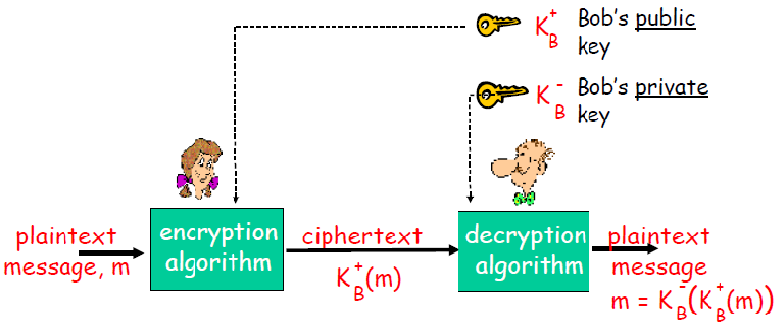
\includegraphics[width=1\linewidth]{Figures/publickeyex.png}
	\caption{Asymmetric Key Encryption}
	\label{fig:asy}
\end{figure}

\subsection{Authenticated Encryption}

Authenticated Encryption, AE, differs from encryption in that it offers authenticity and integrity in addition to confidentiality. A solely AE public key function would require the plaintext message, the private key of the sender and the public key of the recipient to encrypt. The recipient uses a function that would require the ciphertext message, the recipient's private key and the sender's public key in order to decrypt, authenticated and check for integrity. During the encryption process a MAC is produced from the encrypted cipher text and sent with the cipher text. The recipient creates the MAC again from the ciphertext and compares this generated MAC to the received MAC. If they are the same then the message is authentic and integrity is sound. 

\subsection{Digital Signature}

This is a mathematical scheme for proving message authenticity, integrity and message non-repudiation. Similarly to asymmetric key encryption a random private key is created with a corresponding public key. The algorithm takes in a message and a private key and creates a hash from them. It then appends that signature to the message. If Alice signs a message in this way, Bob can use another algorithm to verify the message with the Alice's public key and signature. It is important to note that the data is not hidden at this point, it is still in plain text.

\subsection{Nonce}

A cryptographic nonce is some arbitrary data that is used in the encryption process so that the process doesn't produce the same cipher text for the same plain text if repeated. Therefore a nonce can only be used once. It will most likely be random or pseudo random data and it is incorporated into cryptographic systems in some way such that old communications that an attacker may have captured can't be sent again and accepted as normal. The same nonce used to encrypt the message is needed to decrypt the message so the synchronisation of nonces is very important. Some systems use counters as nonces or the nonces on each side are dependent on the same calculation but nonces created in those ways aren't as secure as generating a new nonce randomly as they can easily predicted. 

\subsection{Message Authentication Code}

A MAC is a small piece of information that is used to authenticate a message and prove it's integrity. The MAC algorithm takes in a message and a key and produces a MAC, then the MAC is sent with the message and the receiver runs the algorithm like the sender, with the same message and key, and if the resulting MAC is the same as the received MAC then the message integrity and authentication can be proved. MACs differ to digital signatures in that it does not provide message repudiation.

\subsection{Stream Cipher}

A stream cipher is a symmetric key cipher where the plain text message is combined with a cipher digit stream so that each digit of the data is encrypted individually. The combining operation is an XOR. This can be useful for applications that are constantly sending data, for example streaming encrypted video. 

\section{TweetNaCl}

NaCl or ``Salt`` is a simple to use high-speed library for authenticated encryption. It provides both Asymmetric and Symmetric encryption, authentication and message integrity with SHA-512. The authors are Daniel J. Bernstein, Tanja Lange and Peter Schwabe but at points it does rely on some third part implementations. The API is simple, having only a handful of methods but provides good, high performance security.

It provides everything needed for secure data transmission but unfortunately the library is relatively quite large, the Arduino Due has at it's disposal 512KB flash memory but the full NaCl library is 3MB. Fortunately the same creators along with Bernard van Gastel, Wesley Janssen and Sjaak Smetsers made TweetNaCl. Which is a tiny implementation of NaCl, still providing good performance and good security but with a significantly smaller code size of 40KB. It retains the same protections against timing attacks, cache-timing attacks, has no branches depending on secret data and no array indices depending on secret data. In addition it is thread-safe and has no dynamic memory allocation\cite{tweetnacl}. It is portable and easy to integrate, the library is easily added as it consists of two files, there is no complicated configuration to be set up or any dependencies on external libraries. Because of this compactness it is easy to read and understand it's operation. Although not as fast as NaCl it is still fast enough for most applications. The authors of the library feel that the performance is acceptable as``Most applications can tolerate the 4.2 million cycles that OpenSSL uses on an Ivy Bridge CPU for RSA-2048 decryption, for example, so they can certainly tolerate the 2.5 million cycles that TweetNaCl uses for higher-security decryption (Curve25519).'' \cite{tweetnacl3}.

TweetNaCl is still small after compilation at 11KB thus reducing instruction cache misses. It is a full library and not a set of isolated functions, for this TweetNaCl application, only six functions are needed. For public-key authenticated keypairs \emph{crypto\_box\_keypair}, \emph{crypto\_box} to authenticated encrypt and \emph{crypto\_box\_open} for authenticated decryption. Similarly for signature keypairs \emph{crypto\_sign\_keypair}, to sign messages \emph{crypto\_sign} and to verify signatures \emph{crypto\_sign\_open}. A keypair is a mathematically paired public key and private key. TweetNaCl is open source and the developers encourage it to be used as much as possible. 

Unfortunately the library won't compile as is on a Arduino, one problem is that there is no /dev/random and therefore no randombytes() which means that it can't create random private keys and therefore good keypairs. The Arduinos can generate pseudorandom numbers by generating a seed from an analogue pin which will provide fairly random numbers but it is considered insecure for cryptographic applications to use pseudorandom numbers like that\cite{arduinopseudo}. It is possible to create true random numbers by utilising the truly random nature of atmospheric noise or background radiation but this requires extra components and is outside the scope of this project. Also, as mentioned in the implementation section the Arduino can't use the C library as is, one approach to resolving this is to convert it into a C++ header file and cpp file relationship.

For public key authenticated encryption, TweetNaCl uses three components: Curve25519 Diffie–Hellman key-exchange function, Salsa20 stream cipher for message encryption and Poly1305 for message authentication and integrity. Curve25519 Diffie–Hellman key-exchange function is used to compute the shared secret between sender and receiver using the sender's secret key and receivers public key. Curve25519 is an elliptic curve, which is an approach to public key cryptography that is based on the algebraic structure of elliptic curves over finite fields, used in conjunction with the elliptic curve Diffie-Hellman anonymous key agreement protocol\cite{curve}. For message encryption the Salsa20 stream cipher encrypts a message using the shared secret. Salsa20 uses a pseudorandom function based on add-rotate-xor, bitwise additions and rotation operations. The cipher uses XOR operations, 32-bit addition, mod $2^{32}$ and constant-distance rotation operations on an internal state of sixteen 32-bit words\cite{salsa}. The library uses Poly1305 as it's MAC function\cite{poly}.

For key signature, TweetNaCl has a fourth component, Ed25519 public key signature system. Edwards curve digital signature algorithm is a variant of Schnorr signature based on Twisted Edward curves. It is faster than existing schemes but does not reduce strength of security\cite{ed25}. TweetNaCl gets it's name because the developers tweeted all of the source code in a 100 tweets to prove how small it was.

%explain how the encryption and signature's work. high level overview
% Curve25519 Diffie–Hellman key-exchange function public key
% Ed25519 signature 

\section{Types of attacks}

\subsection{Replay Attack}

When this attack occurs the attacker replays a valid message attempting to cause a legitimate action to be repeated. If Bob wants Alice to provide authentication and she duly provides some encrypted signature to prove her identity. Eve can capture that signature, she does not need to know what the signature is but she knows that it is a signature. She can then connect to Bob and when Bob asks for identification she can use this captured signature to pretend she is Alice. To prevent this attack Alice might use an identifier that is only valid for one use, this could be session tokens or one-time passwords. These attacks are also known as playback attacks.

\subsection{Man in the Middle Attack}
Also known as MITM. In this attack there is an attacker between two parties, Bob and Alice, who wish to communicate. The man in the middle, Eve, changes messages as they are in transit to either pretend that she is the person that the other thinks they are talking to, change the contents of the message or something else. An example is if Alice asks for Bob's public key, Eve can capture that public key, replace it with her own and send that and because Alice has no way to prove that it is Bob's key or not she accepts it. So when Alice sends a message that has been encrypted with what she thinks is Bob's key, Eve can take it, decrypt it with her key, read or change the message before encrypting it with Bob's real public key and sending it to Bob. Alice thought she had encrypted a message with Bob's key and that only Bob would be able to read it but this was not the case.

\subsection{Bit-Flipping Attack}
This is where the attacker can change the cipher text, that was produced by a simple encryption function, in some way that causes a predictable change in the plain text. Eve does not need to know exactly what the plain text is, just some of it or just the format. For example if Alice was to send a message to Bob saying that she owes him £100 and Eve knows at least some of the message format, she can change the number at the end into £900. 

\subsection{Stream Cipher Attack}
If the same key is reused in a stream cipher then it becomes vulnerable. If Alice were to encrypt two messages of the same length with the same key, Eve can take the two encrypted messages and XOR them to produce the message. If one message was longer than the other then Eve could only find out the section of the longer message that was the same length as the shorter.

\section{Timing Attack}
In this type of attack strategy, an attacker measures the time that the system takes to perform some action that depends on the secret data. If the execution time differs because the system is taking different execution paths depending on secret data then it is possible to deduce information about said data. For example the login program in early versions of Unix executed the crypt function only when the login name was recognised. By this, an attacker was able to find out if a login name was correct even if the password wasn't.

\section{Machine to Machine}

M2M refers to the direct communication between two or more devices using any sort of channel. This is a component of IoT and when connected in this way small, low power sensors can transmit their data to another device which can collate, perform analysis or some extra computation or pass the data along again before it reaches a human user. Present day applications include monitoring the health of machinery, digital billboards or sensory networks. An application may possess multiple sensors in a network that pass sensor data to multiple nodes which do some computation, such as adjust machines to correct errors, replenish stock or manage a system and possibly sending information, such as state across the Internet to a human user.

\section{Technologies used}

In this project the Arduino was programmed using C++. The C++ was developed in the Arduino IDE. An Arduino Due, Arduino Uno, DS18S20 temperature sensor, resistor and two Ethernet Shield R2 boards were used. On the server side there is an SQL server, PHP scripts that accept that Arduino data and put it in the SQL database. And a Java web application that uses Java Database Connectivity, JBCD, to access the SQL server and output dynamic HTML when accessed. The Java code was developed using Eclipse Jee Mars. Bitbucket, using Git, was used to remotely store all the software.

\subsection{XAMPP Server}

XAMPP, Apache, MySQL, PHP and Perl come together to form XAMPP which is a free, open source, cross platform, web server stack package for the creation and testing of local server systems that can then be moved easily live systems. This XAMPP used in this project also contains Tomcat.

\subsection{PHP}
PHP is a server-side scripting language used in web development. It is especially suited to server-side applications as it is very portable. PHP code is contained in a file and when the server receives a request, the code is executed by the PHP runtime. It can be used with many OS's, web servers and relational database management systems. It is very common for web hosting providers to support PHP use by their clients.

\subsection{SQL}

Standard Query Language is a special purpose programming language for managing data stored in relational databases. SQL organises data into databases and tables and has operations for inserting, updating, deleting, altering and querying data. The vast majority of the databases in businesses use SQL.

\subsection{Apache Tomcat}

Tomcat is an open source implementation of the Java servlet, JavaServer Pages, Java Expression Language and Java Websocket technologies. It provides the ability to produce dynamic HTML in a pure Java environment. It accepts web application archives, WAR files,  for easy updating of web apps.

\subsection{Hypertext Transfer Protocol}

HTTP is a protocol for the distribution of information across the world wide web. It is the foundation of internet data communication. Clients send HTTP requests in a certain format to servers in order to perform certain actions such as sending data or retrieving it. In this project HTTP/1.1, which is a revision of the original, HTTP/1.0 is utilised. POST and GET requests are used in this project but there are many other request methods.

%JBCD? Accessible through web by port forwarding.
\section{Secure Transmission of Keys}
\label{keydist}

In symmetric key encryption the same secret key is used to encrypt and decrypt messages. If two parties want to create a secure channel, how do they make sure they are using the same private key. How do they share the secret key securely without anyone else having access to it. This problem is known as the key distribution problem. One solution is to meet in person and in private with the person you plan to communicate with and exchange the key there. If the communication is of a diplomatic nature, the bag used to transport the keys can have special legal protection against being opened and this is called a diplomatic bag\cite{dipbag}. Another solution is to send the key over another secure channel that you trust but how can a secure channel be created without first having a shared secret key which you can't be created without first having a shared secret key. Later, public key encryption was developed to solve the problem of passing out shared secret keys. Public keys could now be passed around so parties could encrypt messages and there was little fear that others parties could decrypt those messages unless they were had access to the private key. The private key did not have to be sent anywhere so the risk of it being leaked out was reduced. However the problem wasn't completely solved. How can Alice send her public key to Bob and make sure that Bob received the correct public key. It is possible a MITM attack could occur and Charlie might have interrupted the valid transmission and sent his own public key instead so he could decrypt the messages that Bob had meant only for Alice to see. A solution to this is public key certificates, an electronic document that is used to prove ownership of a public key.  When a user has created a public-private key pair they generate a Certificate Signing Request, CSR, and send it to a Certificate Authority, CA. The CA checks the integrity of the CSR and the users identity. If all is well the CA signs the certificate and sends it back. Now when the user can provide a certificate as proof that the public key is indeed theirs. The recipient of the public key trusts in the CA and the certificate so therefore trusts the public key they have received. The CA is s trusted third party that can be used to verify public keys.
